\chapter{Flexion pure (plane, circulaire)}
\section{Théorie}
	\subsection{Méthode cinématique}
	\begin{wrapfigure}[8]{r}{6.5cm}
	\vspace{-7mm}
	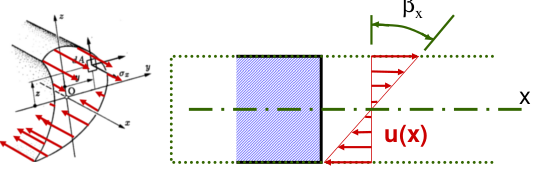
\includegraphics[scale=0.4]{ch4/image1.png}
	\captionof{figure}{ }
	\end{wrapfigure}
	Nous allons cette fois-ci encore utiliser la méthode cinématique, mais 
	avec un autre champ de déplacement :
	\begin{equation}
	u=z\beta_x(x),\qquad v=0,\qquad w=w_0(x).
	\end{equation}
	Il s'agit d'un déplacement axial $u$ variant linéairement en fonction 
	de la coordonnée $z$. Notons $O$, le centre géométrique.
	
	\subsection{Déformations – Contraintes}
		\subsubsection{Déformations}
		$\epsilon_x$ est une fonction linéaire en $z$ dans la section 
		transversale :
		\begin{equation}
		a_{ij} =  \frac{1}{2}\left(\dfrac{\partial u_i}{\partial x_j}+\dfrac{
		\partial u_j}{\partial x_i}\right)
		\end{equation}
		Forcement, les composantes autres que $\epsilon_x$ et $\gamma_{xz}$ 
		sont nulles
		\begin{equation}
		\epsilon_x = z\dfrac{\partial \beta_x}{\partial x}\qquad \gamma_{xz} = 
		\beta_x + \dfrac{\partial w_0}{\partial x}
		\end{equation}
		Par contre, ce $\gamma_{xz}$ non-nul est un peu casse-cojones. Du coup, 
		on supposera plus loin que les déformations normales à la section 
		droite restent normales apres la déformation $\rightarrow$ pas de 
		variation d'angle $\rightarrow \gamma_{xz} = 0$. Oui, tu l'as reconnu ! 
		C'est l'\textit{hypothèse de Bernoulli}.
		
		\subsubsection{Contraintes}
		On conserve la loi de Hooke $\sigma_x = E\epsilon_x$ mais avec 
		l'expression $\epsilon_x$ développée ci-dessus. Dans ce cas, si 
		$E =\ cste$, $\sigma_x$ est une fonction linéaire de $z$ dans la 
		section transversale. On néglige encore Poisson et plus tard, on 
		s'intéressera à $\tau_{xz}$.
		
	\subsection{Éléments de réduction : section homogène}
	Commençons par calculer la réaction normale (pour une section homogène, 
	$E =\ cste$) :
	\begin{equation}
	N = \int_A\sigma_x\ dA\qquad\Leftrightarrow\qquad N = E\dfrac{\partial 
	\beta_x}{\partial x}\int_A z\ dA
	\end{equation}
	Mon rêve est d'avoir $N=0$. C'est possible si $\int_A z\ dA=0$. Comme 
	nous n'avons que des forces normales, les autres résultantes sont 
	trivialement nulles, de même pour le moment selon $x$
			\begin{wrapfigure}[7]{l}{6.5cm}
	\vspace{-5mm}
	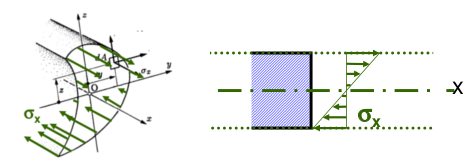
\includegraphics[scale=0.45]{ch4/image2.png}
	\captionof{figure}{ }
	\end{wrapfigure}
	\begin{equation}
	\begin{array}{ll}
	R_y = \int_A \tau_{xy}\ dA &\Longrightarrow T_y = 0\\
	\text{Similairement : }&\Longrightarrow T_z = 0\\
	C_x = \int_A(\tau_{xz}y-\tau_{xy}z)\ dA &\Longrightarrow M_x=0
	\end{array}
	\end{equation}
	Calculons maintenant le moment selon $y$ (signe à adapter selon les 
	convention) : 
	\begin{equation}
	C_y = \int_A \sigma_xz\ dA\qquad\Longrightarrow\qquad M_y = E\dfrac{
	\partial \beta_x}{\partial x}\underbrace{\int_Az^2\ dA}_{I_{zz}}
	\end{equation}
	On reconnaît la définition du moment d’inertie par rapport à l'axe 
	$y$, aussi appelé $I_y$ :
	\begin{equation}
	M_y = E\dfrac{\partial\beta_x}{\partial x}I_{zz}
	\end{equation}
	Faisons de même pour le moment en $z$ :
	\begin{equation}
	C_z = \int_A \sigma_xy\ dA\qquad\Longrightarrow\qquad M_z = E\dfrac{
	\partial \beta_x}{\partial x}\int_Ayz\ dA
	\end{equation}	
	Notre rêve (oui, encore) est que $M_z=0$. Ce sera le cas si $\int_A 
	yz\ dA = 0$.\\
	
		\subsubsection{Comment faire pour que ces intégrales soient nulles ?}
		Oui, comment?! Il suffit de considérer $y$ et $z$ comme les 
		\textbf{axes principaux} d’inertie de la section transversale : ceci 
		défini l’origine des axes, à savoir le \textbf{centre géométrique}
		
		\subsubsection{En résumé}
		La poutre est soumise uniquement à un moment fléchissant $M_y$ (ou 
		$M_z$ si l'on considère l'autre axe).
		Pour une distribution de la contrainte axiale linéaire en fonction 
		de $z$ :
		\begin{equation}
		\epsilon_x = z\dfrac{\partial \beta_x}{\partial x},\qquad \sigma_x 
		= E\epsilon_x,\qquad M_y = E\dfrac{\partial \beta_x}{\partial x}I_y.
		\end{equation}
		Par remplacement successif, on peut trouver $\sigma_x$ :
		\begin{equation}
		\left.\begin{array}{ll}
		\sigma_x &= Ez\dfrac{\partial \beta_x}{\partial x}\\
		E\dfrac{\partial\beta_x}{\partial x} &= \dfrac{M_y}{I_y}
		\end{array}\right\}\Longrightarrow\quad \sigma_x = \dfrac{M_y}{I_y}z
		\end{equation}
		Si on considère une flexion selon l'autre axe, on trouvera de 
		façon similaire $\sigma_x = \dfrac{M_z}{I_z}y$.
		
	\subsection{Pour une structure plane}
	Considérons le plan $xz$ de la structure. Si :
	\begin{itemize}
	\item[$\bullet$] $y$ est perpendiculaire à $xz$
	\item[$\bullet$] $y$ est un axe principal d'inertie des sections planes 
	(poutres)
	\item[$\bullet$] le moment fléchissant $M_y$ est appliqué selon $y$
	\end{itemize}		
	Alors ce moment $M$ provoque un déplacement de flexion \textbf{dans} le 
	plan $xz \longrightarrow$ il n'y a pas d'effort normal ($N=0$).
	
	\subsection{Synthèse}
\vspace{-1cm}
	\begin{wrapfigure}[7]{r}{3.5cm}
	\vspace{-2mm}
	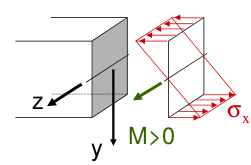
\includegraphics[scale=0.45]{ch4/image3.png}
	\captionof{figure}{ }
	\end{wrapfigure}\ \\
	
	\retenir{Si un axe principal d'inertie de la section transversale est 
	perpendiculaire au plan d'une structure, un moment $M$ perpendiculaire 
	au plan de la structure provoque une flexion dans le plan de la structure}\ \\
	La relation $\sigma_x=\dfrac{M}{I}y$ est valable \textbf{même} sans 
	l'hypothèse de Bernoulli.
	
\section{Relations particulières}
	\subsection{Module de flexion $\leftrightarrow$ moment d’inertie}
	Une section possède deux caractéristiques importantes : 
	\begin{enumerate}
	\item \textit{Le module de flexion}.\\
	La plus grande valeur pour la contrainte correspond à la fibre la plus 
	éloignée de l'axe neutre. Pour une valeur de $M$, on peut 
	diminuer $\sigma_x^{max}$ en augmentant $I/y_{max}$.
	\begin{equation}
	\sigma_x^{max} = \dfrac{M}{I}y_{max},\qquad M=\dfrac{I}{y_{max}}\sigma_x^{
	max},\qquad \text{module de flexion : }\quad \dfrac{I}{y_{max}}
	\end{equation}
	\danger Augmenter $I$ augmente aussi $y_{max}$.
	
	\item \textit{Le moment d'inertie}.\\
	La flèche d'une poutre dépend de $\dfrac{1}{EI}$. Pour diminuer la flèche, 
	on choisira une section à $I$ élevé.
	\end{enumerate}
	Il faut donc choisir des sections ayant des valeurs élevées de $I$ et 
	de $I/y_{max}$ sans augmenter $y_{max}$. En pratique, il y a évidemment 
	d'autres critères de dimensionnement.
	
\section{Bernoulli}
	\subsection{Hypothèse de Bernoulli}
	\begin{wrapfigure}[11]{l}{10.5cm}
	\vspace{-5mm}
	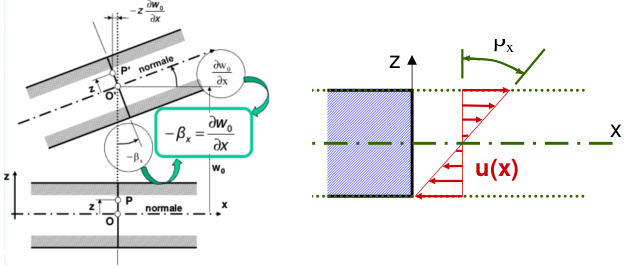
\includegraphics[scale=0.45]{ch4/image4.png}
	\captionof{figure}{ }
	\end{wrapfigure}
	Considérons toujours notre déplacement $u=z\beta_x(x), v=0,w=w_0(x)$.	
	Nous avions 
	\begin{equation}
	\gamma_{xz} = \beta_x+\dfrac{\partial w_0}{\partial x}
	\end{equation}
	L'\textbf{hypothèse de Bernoulli} à pour but de considérer $\gamma_{xz}$ 
	nul, c'est-à-dire :
	\begin{equation}
	\gamma_{xz} = 0\qquad\Longrightarrow\qquad \beta_x = -\dfrac{\partial w_0}{
	\partial x}
	\end{equation}
	 
	\newpage
	\subsection{Les contraintes (sous cette hypothèse)}
		\subsubsection{Contraintes}
		En considérant le même déplacement et notre hypothèse fétiche, nous 
		avons : $\gamma_{xz} = 0 \Longrightarrow \beta_x = -\dfrac{\partial w_0}{
		\partial x}$. On a également
		\begin{equation}
		\tau_{xz} = G\gamma_{xz}
		\end{equation}
		Il en résulte que $\tau_{xz}=0$ implique que l'effort tranchant $T_z$ soit 
		nul et donc $M_y =\ cste$ car 
		\begin{equation}
		\dfrac{dM_y}{dx} = T_z
		\end{equation}
		
	\subsection{Relation "moment-courbure"}
	Les slides (20-21) ont été lâchement passés. A connaître ? 
	
\section{Produit d'inertie}
	\subsection{Axes principaux d'inertie}
	Ils ont deux propriétés :
	\begin{enumerate}
	\item Leur origine est au centre géométrique
	\item Leur orientation est telle que le produit d’inertie est nul
	\end{enumerate}
	On peut les calculer de façon analytique ("Beurk, pas dans ce cours"), 
	où avec le cercle de Mohr.
	
	\subsubsection{Calcul de moments d'intertie}
	Soit par calcul (No!), par logiciel, tables, \dots Il est possible de les 
	obtenir avec les tables et le théorème de Steiner. Je ne détaille pas ça 
	ici, cf. \textit{Mécanique rationnelle II}.
	




